\documentclass[12pt,a4paper]{article}

% --- GÓI HỖ TRỢ TIẾNG VIỆT VÀ FONT ---
\usepackage[utf8]{inputenc}
\usepackage[vietnamese]{babel}
\usepackage{times}
\usepackage{graphicx}
\graphicspath{{figures/}}

% --- CĂN CHỈNH LỀ VÀ KHOẢNG CÁCH ---
\usepackage[left=2.5cm, right=2cm, top=2.5cm, bottom=2.5cm]{geometry}
\usepackage{indentfirst}
\usepackage{setspace}
\setstretch{1.2}
\usepackage{mdframed}
\usepackage{amsmath}
\usepackage{amssymb}
\usepackage{float}
\usepackage{array}
\usepackage{tabularx}
\usepackage{booktabs}
\usepackage{xcolor}
\usepackage{listings}

% Định nghĩa bảng màu code
\definecolor{codegreen}{rgb}{0.13, 0.55, 0.13}    % Màu chú thích (comment)
\definecolor{codepurple}{rgb}{0.58, 0, 0.82}      % Màu chuỗi ký tự (string)
\definecolor{codeblue}{rgb}{0.0, 0.2, 0.8}        % Màu từ khóa (keywords)
\definecolor{backcolour}{rgb}{0.97, 0.97, 0.97}   % Màu nền nhẹ
\definecolor{linegray}{rgb}{0.5, 0.5, 0.5}        % Màu số dòng

\lstdefinestyle{scilabstyle}{
    backgroundcolor=\color{backcolour},
    commentstyle=\color{codegreen}\itshape,
    keywordstyle=\color{codeblue}\bfseries,
    numberstyle=\tiny\color{linegray},
    stringstyle=\color{codepurple},
    basicstyle=\ttfamily\footnotesize,
    breakatwhitespace=false,
    breaklines=true,
    breakindent=15pt,
    postbreak=\mbox{\textcolor{linegray}{$\hookrightarrow$}\space},
    captionpos=b,
    keepspaces=true,
    numbers=left,
    numbersep=8pt,
    showspaces=false,
    showstringspaces=false,
    showtabs=false,
    tabsize=2,
    frame=single,
    rulecolor=\color{black!15},
    xleftmargin=1.5em,
    framexleftmargin=1.5em
}

% Khung kết quả console Scilab
\lstdefinestyle{consolestyle}{
    backgroundcolor=\color{white},
    basicstyle=\ttfamily\footnotesize,
    frame=single,
    rulecolor=\color{black!40},
    numbers=none,
    keepspaces=true,
    showstringspaces=false,
    xleftmargin=4em,
    xrightmargin=4em,
    title={\footnotesize\textsf{Scilab 2026.1.0 Console}}
}

% Khung đề bài dùng chung cho các bài tập
\mdfdefinestyle{exbox}{
    linewidth=0.8pt,
    linecolor=black,
    backgroundcolor=white,
    innertopmargin=10pt,
    innerbottommargin=10pt,
    innerleftmargin=12pt,
    innerrightmargin=12pt,
    skipabove=10pt,
    skipbelow=10pt
}

% --- GÓI HỖ TRỢ ĐƯỜNG DẪN VÀ THAM KHẢO ---
\usepackage{hyperref}
\hypersetup{
    colorlinks=true,
    linkcolor=black,
    urlcolor=blue,
    citecolor=black
}

% Ký hiệu mũi tên đánh dấu gốc tọa độ n = 0
\newcommand{\org}[1]{\underset{\uparrow}{#1}}

% --- THIẾT KẾ PHẦN TIÊU ĐỀ BÁO CÁO ---
\title{
    \vspace{-1.5cm}
    \large\textbf{Xử Lý Tín Hiệu Số} \\
    \normalsize HK261 \quad -- \quad CO2036 \\[1em]
    \Large\textbf{BÀI THỰC HÀNH 4 XỬ LÝ TÍN HIỆU SỐ}
}

\author{
    \textbf{Trần Minh Quang} -- \textbf{2412855}
}

\date{23/10/2026}

\begin{document}

\maketitle

% --- PHẦN TỔNG QUAN ---
\begin{abstract}
\noindent\textbf{Tổng Quan:} Bài thực hành 4 gồm ba bài tính biến đổi Z và miền hội tụ (ROC), hai bài tìm hiểu thư viện xử lý âm thanh và ảnh trong Scilab kèm demo trên dữ liệu thật, và hai bài về tích chập tuyến tính, tích chập vòng bằng phương pháp gập--dịch và phương pháp ma trận. Kết quả mô phỏng trên Scilab đều khớp với tính toán giải tích.
\end{abstract}

\vspace{0.5cm}

% --- NỘI DUNG CHÍNH ---
\section{Giới Thiệu}
Biến đổi Z là công cụ chính để phân tích tín hiệu và hệ thống rời rạc: nó biến phép tích chập trong miền thời gian thành phép nhân đa thức, và miền hội tụ cho biết tín hiệu là nhân quả, phản nhân quả hay hai phía. Bên cạnh phần lý thuyết, bài thực hành này cho em làm quen với việc xử lý dữ liệu thật trong Scilab (một đoạn âm thanh và một bức ảnh), đồng thời mở rộng hàm tích chập đã viết ở Lab 3 sang phương pháp ma trận và tích chập vòng. Công cụ sử dụng là Scilab 2026.1.0.

\section{Mục Tiêu}
\begin{itemize}
    \item \textbf{Về lý thuyết:} tính được biến đổi Z và xác định ROC của tín hiệu hữu hạn, nhân quả và hai phía; hiểu điều kiện hội tụ của tổng tích chập và ý nghĩa của tích chập vòng.
    \item \textbf{Về kỹ năng:} tìm hiểu các hàm và toolbox xử lý âm thanh, ảnh có trong Scilab; hiện thực tích chập tuyến tính và tích chập vòng bằng hai cách khác nhau.
    \item \textbf{Về trực quan hóa:} vẽ dạng sóng, phổ biên độ, ảnh và histogram; vẽ tín hiệu vào, ra và năng lượng trên cùng một figure.
\end{itemize}

\section{Phương Pháp}
\begin{itemize}
    \item \textbf{Bài 1--3:} tính trực tiếp từ định nghĩa $X(z) = \sum_{n=-\infty}^{\infty} x(n) z^{-n}$, dùng tổng cấp số nhân để tìm dạng đóng và điều kiện hội tụ của từng thành phần; ROC của tổng là giao các ROC thành phần.
    \item \textbf{Bài 4--5:} tìm hiểu các hàm có sẵn và toolbox (qua ATOMS), sau đó viết script demo. Dữ liệu dùng là đoạn âm thanh tiếng mèo kêu grừ dài 4 giây (nguồn: pixabay.com) và ảnh chú chó nhà em, được thu nhỏ còn $384 \times 512$ pixel.
    \item \textbf{Bài 6--7:} tính tay bằng bảng gập--dịch và bằng phép nhân ma trận, sau đó hiện thực cả hai cách trên Scilab, đối chiếu với nhau và với hàm \texttt{conv} có sẵn.
\end{itemize}
Các tín hiệu hữu hạn được biểu diễn giống Lab 3: một vector giá trị và chỉ số gốc tọa độ, phần tử thứ $i$ ứng với thời điểm $n = i - \text{origin}$.

\section{Nội Dung Thực Hành}

% =====================================================================
\subsection{Bài tập 1 -- Biến đổi Z của tín hiệu hữu hạn}
\begin{mdframed}[style=exbox]
\noindent\textbf{Bài tập 1.} Tìm biến đổi Z và miền hội tụ (ROC) của tín hiệu
\[
    x(n) = 2\delta(n+2) - \delta(n+1) + 2\delta(n) - 3\delta(n-1) + 4\delta(n-2).
\]
\end{mdframed}

\noindent\textbf{Cơ sở lý thuyết và tính toán:}

Áp dụng cặp biến đổi $\delta(n - n_0) \overset{Z}{\longleftrightarrow} z^{-n_0}$ (hội tụ mọi nơi trừ $z = 0$ khi $n_0 > 0$ và trừ $z = \infty$ khi $n_0 < 0$) cùng tính tuyến tính:
\begin{equation}
    X(z) = 2z^{2} - z + 2 - 3z^{-1} + 4z^{-2}.
\end{equation}
Tín hiệu có chiều dài hữu hạn nên tổng luôn hội tụ, ngoại trừ hai điểm: các số hạng $z^{2}$, $z$ (ứng với $n < 0$) tiến ra vô cùng khi $z \to \infty$, còn các số hạng $z^{-1}$, $z^{-2}$ (ứng với $n > 0$) tiến ra vô cùng khi $z \to 0$. Do đó
\[
    \text{ROC: } 0 < |z| < \infty.
\]

% =====================================================================
\subsection{Bài tập 2 -- Tổng hai tín hiệu nhân quả}
\begin{mdframed}[style=exbox]
\noindent\textbf{Bài tập 2.} Tìm biến đổi Z và ROC của $x(n) = 0.5^{n} u(n) + 0.4^{n} u(n)$.
\end{mdframed}

\noindent\textbf{Cơ sở lý thuyết và tính toán:}

Với tín hiệu nhân quả $a^n u(n)$:
\[
    \sum_{n=0}^{\infty} a^n z^{-n} = \sum_{n=0}^{\infty} \left(a z^{-1}\right)^n = \frac{1}{1 - a z^{-1}}, \qquad \text{hội tụ khi } |a z^{-1}| < 1 \iff |z| > |a|.
\]
Áp dụng cho từng thành phần:
\[
    0.5^n u(n) \overset{Z}{\longleftrightarrow} \frac{1}{1 - 0.5 z^{-1}},\ |z| > 0.5;
    \qquad
    0.4^n u(n) \overset{Z}{\longleftrightarrow} \frac{1}{1 - 0.4 z^{-1}},\ |z| > 0.4.
\]
Cộng lại và quy đồng:
\begin{equation}
    X(z) = \frac{1}{1 - 0.5 z^{-1}} + \frac{1}{1 - 0.4 z^{-1}} = \frac{2 - 0.9 z^{-1}}{(1 - 0.5 z^{-1})(1 - 0.4 z^{-1})}.
\end{equation}
ROC là giao của hai miền: $|z| > 0.5$. Đây là phần ngoài của đường tròn đi qua cực có bán kính lớn nhất, đúng với tính chất của tín hiệu nhân quả. Hệ có hai cực tại $z = 0.5$, $z = 0.4$ và hai không điểm tại $z = 0$, $z = 0.45$.

% =====================================================================
\subsection{Bài tập 3 -- Tín hiệu hai phía}
\begin{mdframed}[style=exbox]
\noindent\textbf{Bài tập 3.} Tìm biến đổi Z và ROC của $x(n) = 0.5^{n} u(n) + 0.9^{n} u(-n-1)$.
\end{mdframed}

\noindent\textbf{Cơ sở lý thuyết và tính toán:}

Thành phần thứ nhất là tín hiệu nhân quả, tương tự Bài tập 2:
\[
    0.5^n u(n) \overset{Z}{\longleftrightarrow} \frac{1}{1 - 0.5 z^{-1}}, \qquad |z| > 0.5.
\]
Thành phần thứ hai là tín hiệu \emph{phản nhân quả} (chỉ khác 0 khi $n \le -1$). Đặt $m = -n$:
\[
    \sum_{n=-\infty}^{-1} 0.9^n z^{-n} = \sum_{m=1}^{\infty} \left(\frac{z}{0.9}\right)^m = \frac{z/0.9}{1 - z/0.9} = \frac{z}{0.9 - z} = -\frac{1}{1 - 0.9 z^{-1}},
\]
hội tụ khi $|z/0.9| < 1 \iff |z| < 0.9$. Cộng hai thành phần:
\begin{equation}
    X(z) = \frac{1}{1 - 0.5 z^{-1}} - \frac{1}{1 - 0.9 z^{-1}} = \frac{-0.4\, z^{-1}}{(1 - 0.5 z^{-1})(1 - 0.9 z^{-1})}.
\end{equation}
ROC là giao của hai miền, tức vành khuyên
\[
    \text{ROC: } 0.5 < |z| < 0.9.
\]
Vì $0.5 < 0.9$ nên vành khuyên này khác rỗng và biến đổi Z tồn tại. Đây là đặc trưng của tín hiệu hai phía: ROC nằm giữa hai cực, cực $0.5$ thuộc phần nhân quả ở phía trong, cực $0.9$ thuộc phần phản nhân quả ở phía ngoài. Nếu đổi chỗ hai cơ số (phần nhân quả có cơ số lớn hơn) thì giao sẽ rỗng và $X(z)$ không tồn tại.

% =====================================================================
\subsection{Bài tập 4 -- Thư viện xử lý âm thanh trong Scilab}
\begin{mdframed}[style=exbox]
\noindent\textbf{Bài tập 4.} Tìm hiểu các thư viện hoặc toolbox có sẵn trong Scilab để xử lý dữ liệu âm thanh.
\end{mdframed}

\noindent\textbf{1. Tìm hiểu thư viện:}

Scilab có sẵn các hàm xử lý âm thanh ngay trong bản cài đặt chuẩn, không cần cài thêm toolbox:
\begin{table}[H]
\centering
\small
\begin{tabularx}{0.85\linewidth}{>{\ttfamily}l X}
\toprule
\textrm{\textbf{Hàm}} & \textbf{Chức năng} \\
\midrule
wavread / wavwrite & Đọc / ghi file \texttt{.wav} \\
sound / playsnd & Phát âm thanh ra loa \\
analyze, mapsound & Vẽ phổ tần số, spectrogram \\
fft & Tính phổ của tín hiệu \\
\bottomrule
\end{tabularx}
\caption{Một số hàm xử lý âm thanh có sẵn trong Scilab}
\end{table}

\noindent\textbf{2. Demo và mã nguồn:}

Em dùng đoạn âm thanh tiếng mèo kêu grừ dài 4 giây (nguồn: \url{https://pixabay.com}), đã chuyển từ \texttt{.mp3} sang \texttt{.wav} vì \texttt{wavread} chỉ đọc được file \texttt{.wav}. Script đọc file, vẽ dạng sóng theo thời gian và phổ biên độ tính bằng \texttt{fft}.

\lstinputlisting[language=Scilab, style=scilabstyle]{../scilab_src/Ex_4.4.sci}

\noindent\textbf{3. Kết quả và nhận xét:}
\begin{lstlisting}[style=consolestyle]
--> exec('Ex_4.4.sci', -1)
   16.
  "so bit moi mau ="
   16000.
  "tan so lay mau fs ="
   4.
  "thoi luong (s) ="
\end{lstlisting}

\begin{figure}[H]
    \centering
    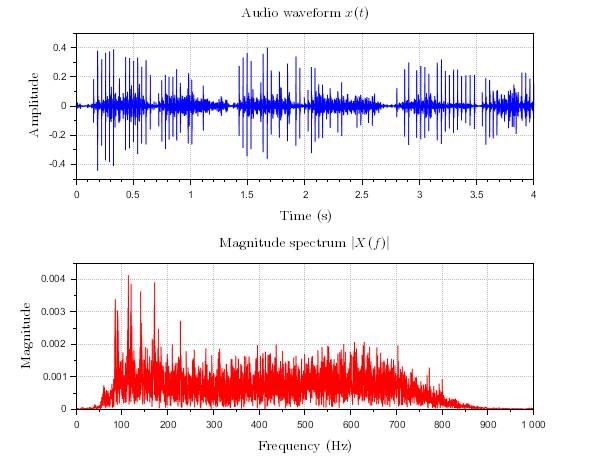
\includegraphics[width=0.9\linewidth]{ex4.4_0.png}
    \caption{Dạng sóng và phổ biên độ của đoạn âm thanh tiếng mèo kêu grừ}
    \label{fig:ex44}
\end{figure}

File âm thanh được đọc đúng: 16 bit mỗi mẫu, tần số lấy mẫu 16 kHz, dài 4 giây. Dạng sóng (Hình~\ref{fig:ex44}, trên) gồm nhiều xung ngắn lặp lại đều đặn, đúng với đặc điểm của tiếng grừ. Phổ biên độ (dưới) cho thấy năng lượng tập trung ở vùng tần số thấp, khoảng 80--800 Hz, với đỉnh lớn nhất quanh 114 Hz.

% =====================================================================
\subsection{Bài tập 5 -- Thư viện xử lý ảnh trong Scilab}
\begin{mdframed}[style=exbox]
\noindent\textbf{Bài tập 5.} Tìm hiểu các thư viện hoặc toolbox xử lý ảnh trong Scilab. Sau đó thực hiện một ví dụ hoặc demo minh họa một thao tác đơn giản (ví dụ: hiển thị histogram, cân bằng histogram, làm mờ, đóng dấu watermark) trên một ảnh số.
\end{mdframed}

\noindent\textbf{1. Tìm hiểu thư viện:}

Scilab chuẩn không có hàm đọc ảnh, cần cài thêm toolbox qua ATOMS. Toolbox phổ biến hiện nay là \textbf{IPCV}, cài bằng \texttt{atomsInstall("IPCV")}, cung cấp các hàm \texttt{imread}, \texttt{imshow}, \texttt{imhist}, \texttt{imfilter}, \dots; toolbox cũ hơn là \textbf{SIVP} nhưng không còn được cập nhật. Để script chạy được cả khi chưa cài toolbox, em tự viết hàm \texttt{read\_pgm} đọc ảnh xám dạng \texttt{.pgm}, còn các phép xử lý chỉ dùng hàm có sẵn của Scilab (\texttt{conv2}, \texttt{cumsum}, \texttt{Matplot}).

\noindent\textbf{2. Các phép xử lý thực hiện:}
\begin{itemize}
    \item \textbf{Histogram:} đếm số pixel ở mỗi mức xám từ 0 đến 255.
    \item \textbf{Cân bằng histogram:} ánh xạ mức xám qua hàm phân bố tích lũy để trải đều các mức xám, giúp tăng độ tương phản.
    \item \textbf{Làm mờ:} tích chập ảnh với bộ lọc trung bình $5 \times 5$.
    \item \textbf{Watermark:} giấu một ảnh nhị phân vào bit thấp nhất (LSB) của mỗi pixel, sau đó tách lại.
\end{itemize}

\noindent\textbf{3. Mã nguồn thực thi trên Scilab:}
\lstinputlisting[language=Scilab, style=scilabstyle]{../scilab_src/Ex_4.5.sci}

\noindent\textbf{4. Kết quả và nhận xét:}

\begin{figure}[H]
    \centering
    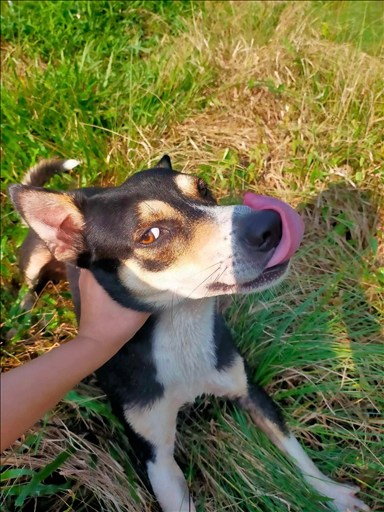
\includegraphics[width=0.38\linewidth]{ex4.5_color.jpg}
    \caption{Ảnh gốc dùng cho demo (Credit: Chó ở nhà em)}
    \label{fig:ex45color}
\end{figure}

\begin{lstlisting}[style=consolestyle]
--> exec('Ex_4.5.sci', -1)
   1.
  "sai lech lon nhat sau khi giau watermark ="
  T
  "tach watermark dung ="
\end{lstlisting}

\begin{figure}[H]
    \centering
    \begin{minipage}{0.3\linewidth}
        \centering
        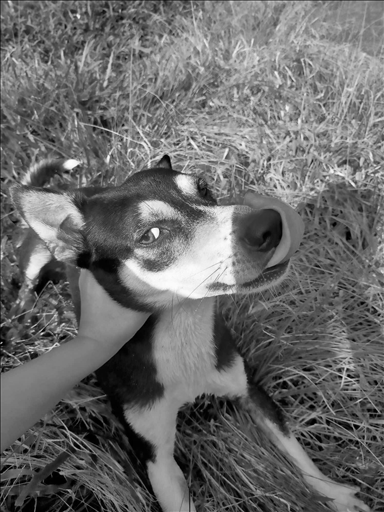
\includegraphics[width=\linewidth]{ex4.5_gray.png}
        \\ \small (a) Ảnh xám gốc
    \end{minipage}
    \hfill
    \begin{minipage}{0.3\linewidth}
        \centering
        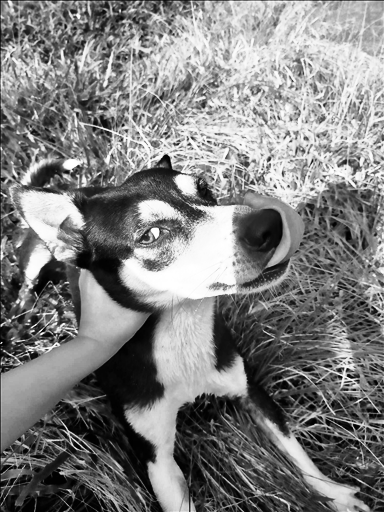
\includegraphics[width=\linewidth]{ex4.5_eq.png}
        \\ \small (b) Cân bằng histogram
    \end{minipage}
    \hfill
    \begin{minipage}{0.3\linewidth}
        \centering
        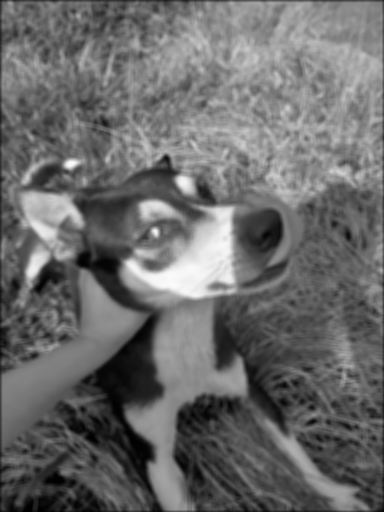
\includegraphics[width=\linewidth]{ex4.5_blur.png}
        \\ \small (c) Làm mờ $5 \times 5$
    \end{minipage}
    \\[1em]
    \begin{minipage}{0.3\linewidth}
        \centering
        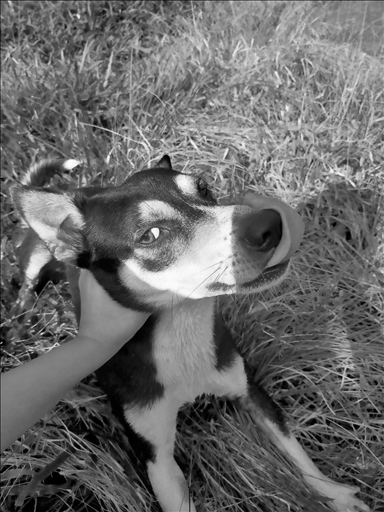
\includegraphics[width=\linewidth]{ex4.5_marked.png}
        \\ \small (d) Ảnh đã giấu watermark
    \end{minipage}
    \hspace{0.04\linewidth}
    \begin{minipage}{0.3\linewidth}
        \centering
        
\includegraphics[width=\linewidth]{ex4.5_wm.png}
        \\ \small (e) Watermark tách ra
    \end{minipage}
    \caption{Ảnh xám gốc và kết quả các phép xử lý}
    \label{fig:ex45all}
\end{figure}

\begin{figure}[H]
    \centering
    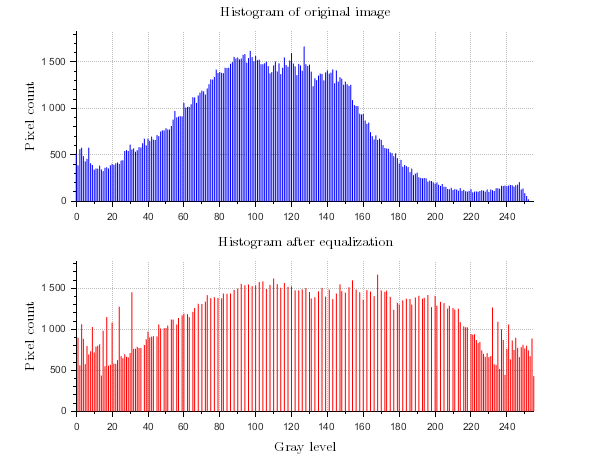
\includegraphics[width=0.8\linewidth]{ex4.5_1.png}
    \caption{Histogram của ảnh trước (trên) và sau (dưới) khi cân bằng}
    \label{fig:ex45hist}
\end{figure}

Nhận xét:
\begin{itemize}
    \item \textbf{Cân bằng histogram:} histogram ảnh gốc dồn chủ yếu ở các mức xám trung bình, sau khi cân bằng thì trải đều hơn trên toàn dải 0--255 (Hình~\ref{fig:ex45hist}). Ảnh (b) có độ tương phản cao hơn, cỏ và lông đen rõ chi tiết hơn so với ảnh gốc (a).
    \item \textbf{Làm mờ:} ở ảnh (c), các chi tiết nhỏ như sợi cỏ, ria mép bị nhòe đi, còn các vùng lớn vẫn giữ hình dạng.
    \item \textbf{Watermark:} ảnh (d) nhìn không khác gì ảnh gốc vì mỗi pixel chỉ thay đổi tối đa 1 mức xám (console in ra 1), và watermark tách ra (e) đúng với watermark đã giấu (console in \texttt{T}).
\end{itemize}

% =====================================================================
\subsection{Bài tập 6 -- Tích chập tuyến tính}
\begin{mdframed}[style=exbox]
\noindent\textbf{Bài tập 6.} Cho hai tín hiệu rời rạc $x(n)$, $h(n)$, $n = 0, \pm 1, \pm 2, \dots$ xác định trên toàn trục $n$. Tích chập tuyến tính của chúng là
\[
    y(n) = \sum_{k=-\infty}^{\infty} h(k)\, x(n-k).
\]
\begin{itemize}
    \item Suy ra biểu thức của $y(n)$ sao cho $y(n)$ hội tụ trong các trường hợp: (i) cả $h(n)$ và $x(n)$ đều nhân quả; (ii) hệ có đáp ứng xung hữu hạn, $h(n) = 0$ với $n < 0$ hoặc $n > M$.
    \item Giả sử trường hợp (ii) xảy ra, tính $y(n)$ với $x(n) = [\org{1}, 2, -3, 2, 1]$ và $h(n) = [\org{1}, 0, -1]$ bằng phương pháp gập và dịch, hiện thực bằng Scilab.
    \item Tính lại $y(n)$ bằng phương pháp ma trận, hiện thực bằng Scilab.
    \item Vẽ $x(n)$, $y(n)$ và năng lượng của các tín hiệu trên cùng một hình.
\end{itemize}
\end{mdframed}

\noindent\textbf{1. Cơ sở lý thuyết và tính toán:}

\textbf{(i) Cả $h(n)$ và $x(n)$ đều nhân quả.} Vì $h(k) = 0$ với $k < 0$ và $x(n-k) = 0$ khi $n - k < 0$, tức $k > n$, nên chỉ các số hạng $0 \le k \le n$ còn lại:
\begin{equation}
    y(n) =
    \begin{cases}
        \displaystyle\sum_{k=0}^{n} h(k)\, x(n-k), & n \ge 0, \\[2ex]
        0, & n < 0.
    \end{cases}
\end{equation}
Với mỗi $n$, tổng chỉ có $n + 1$ số hạng hữu hạn nên $y(n)$ luôn xác định (hội tụ), và $y(n)$ cũng là tín hiệu nhân quả.

\textbf{(ii) Hệ FIR.} Vì $h(k) = 0$ ngoài đoạn $0 \le k \le M$:
\begin{equation}
    y(n) = \sum_{k=0}^{M} h(k)\, x(n-k).
\end{equation}
Mỗi $y(n)$ chỉ là tổng của $M + 1$ số hạng nên luôn hội tụ với mọi $n$. Hơn nữa, nếu $x(n)$ bị chặn, $|x(n)| \le B$, thì $|y(n)| \le B \sum_{k=0}^{M} |h(k)| < \infty$, nghĩa là hệ FIR luôn ổn định BIBO.

\textbf{Phương pháp gập và dịch.} Ở đây $h(n) = \delta(n) - \delta(n-2)$, $M = 2$, nên $y(n) = x(n) - x(n-2)$. Thực hiện theo các bước: gập $h(k)$ thành $h(-k) = [-1, 0, \org{1}]$, dịch đi $n$ mẫu thành $h(n-k)$, nhân từng mẫu với $x(k)$ rồi cộng lại. Tín hiệu ra có chiều dài $L_y = 5 + 3 - 1 = 7$ và bắt đầu tại $n = 0 + 0 = 0$:
\begin{table}[H]
\centering
\begin{tabular}{c|c|c}
\toprule
$n$ & Các mẫu $x(k)$ chồng lên $h(n-k)$ & $y(n)$ \\
\midrule
0 & $x(0)h(0) = 1 \cdot 1$ & $1$ \\
1 & $x(1)h(0) + x(0)h(1) = 2 + 0$ & $2$ \\
2 & $x(2)h(0) + x(1)h(1) + x(0)h(2) = -3 + 0 - 1$ & $-4$ \\
3 & $x(3)h(0) + x(2)h(1) + x(1)h(2) = 2 + 0 - 2$ & $0$ \\
4 & $x(4)h(0) + x(3)h(1) + x(2)h(2) = 1 + 0 + 3$ & $4$ \\
5 & $x(4)h(1) + x(3)h(2) = 0 - 2$ & $-2$ \\
6 & $x(4)h(2) = -1$ & $-1$ \\
\bottomrule
\end{tabular}
\caption{Tính tích chập tuyến tính bằng phương pháp gập và dịch}
\end{table}
\noindent Vậy $y(n) = [\org{1}, 2, -4, 0, 4, -2, -1]$.

\textbf{Phương pháp ma trận.} Viết $\mathbf{y} = \mathbf{H}\mathbf{x}$, trong đó $\mathbf{H}$ là ma trận Toeplitz kích thước $L_y \times L_x = 7 \times 5$. Cột thứ $j$ của $\mathbf{H}$ là $h(n)$ dịch xuống $j - 1$ mẫu:
\[
    \mathbf{y} =
    \begin{bmatrix}
         1 &  0 &  0 &  0 &  0 \\
         0 &  1 &  0 &  0 &  0 \\
        -1 &  0 &  1 &  0 &  0 \\
         0 & -1 &  0 &  1 &  0 \\
         0 &  0 & -1 &  0 &  1 \\
         0 &  0 &  0 & -1 &  0 \\
         0 &  0 &  0 &  0 & -1
    \end{bmatrix}
    \begin{bmatrix} 1 \\ 2 \\ -3 \\ 2 \\ 1 \end{bmatrix}
    =
    \begin{bmatrix} 1 \\ 2 \\ -4 \\ 0 \\ 4 \\ -2 \\ -1 \end{bmatrix}.
\]
Kết quả trùng với phương pháp gập và dịch.

\textbf{Năng lượng.} Với $E = \sum_n |x(n)|^2$:
\[
    E_x = 1 + 4 + 9 + 4 + 1 = 19, \qquad E_y = 1 + 4 + 16 + 0 + 16 + 4 + 1 = 42.
\]

\noindent\textbf{2. Mã nguồn thực thi trên Scilab:}
\lstinputlisting[language=Scilab, style=scilabstyle]{../scilab_src/Ex_4.6.sci}

\noindent\textbf{3. Kết quả mô phỏng và nhận xét:}
\begin{lstlisting}[style=consolestyle]
--> exec('Ex_4.6.sci', -1)
   1.   2.  -4.   0.   4.  -2.  -1.
  "yn (gap va dich) ="
   1.
  "yorigin ="
   1.   2.  -4.   0.   4.  -2.  -1.
  "yn (ma tran) ="
   1.
  "yorigin ="
   1.   2.  -4.   0.   4.  -2.  -1.
  "conv(xn, hn) ="
   19.
  "Ex ="
   42.
  "Ey ="
\end{lstlisting}

\begin{figure}[H]
    \centering
    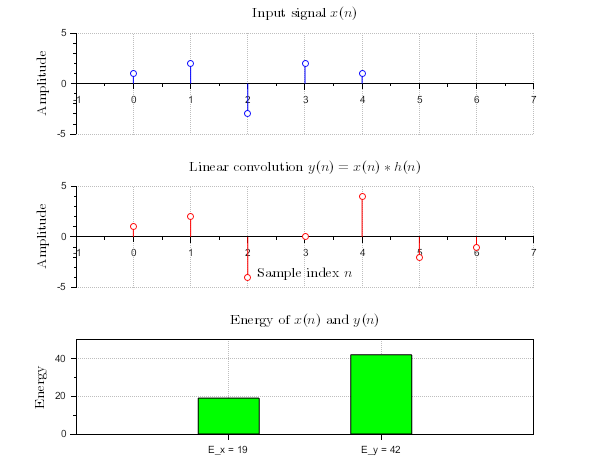
\includegraphics[width=0.85\linewidth]{ex4.6_0.png}
    \caption{Tín hiệu vào $x(n)$, tín hiệu ra $y(n) = x(n) * h(n)$ và năng lượng của hai tín hiệu}
    \label{fig:ex46}
\end{figure}

Hai phương pháp và hàm \texttt{conv} có sẵn của Scilab cho cùng kết quả $[1, 2, -4, 0, 4, -2, -1]$, với gốc tọa độ ở phần tử đầu tiên. Trên Hình~\ref{fig:ex46}, $y(n)$ dài 7 mẫu, kéo dài thêm $M = 2$ mẫu so với $x(n)$. Năng lượng tăng từ $E_x = 19$ lên $E_y = 42$, vì hệ $h(n) = \delta(n) - \delta(n-2)$ cộng thêm một bản trễ đảo dấu của $x(n)$ vào chính nó. Phương pháp gập--dịch phù hợp để hiểu bản chất và tính tay, còn phương pháp ma trận thuận tiện khi lập trình vì chỉ là một phép nhân ma trận--vector.

% =====================================================================
\subsection{Bài tập 7 -- Tích chập vòng}
\begin{mdframed}[style=exbox]
\noindent\textbf{Bài tập 7.} Với tín hiệu tuần hoàn $x(n)$ có chiều dài $N$ và đáp ứng xung $h(n)$ có chiều dài $M$, tích chập vòng giữa $x(n)$ và $h(n)$ được định nghĩa là
\[
    y(n) = \sum_{k=0}^{M-1} h(k)\, x[(n-k) \bmod N].
\]
Giải thích vì sao $y(n)$ có thể được suy ra như vậy.
\begin{itemize}
    \item Tính $y(n)$ với $x(n) = [\org{1}, 2, -3, 2, 1]$ và $h(n) = [\org{1}, 0, -1, -1, 1]$ bằng phương pháp gập và dịch, hiện thực bằng Scilab.
    \item Tính lại $y(n)$ bằng phương pháp ma trận, hiện thực bằng Scilab.
    \item Vẽ $x(n)$, $y(n)$ và năng lượng của các tín hiệu trên cùng một hình.
\end{itemize}
\end{mdframed}

\noindent\textbf{1. Cơ sở lý thuyết và tính toán:}

\textbf{Giải thích công thức.} Xuất phát từ tích chập tuyến tính $y(n) = \sum_{k} h(k)\, x(n-k)$:
\begin{itemize}
    \item $h(n)$ chỉ khác 0 khi $0 \le k \le M-1$, nên tổng chỉ còn $M$ số hạng, từ $k = 0$ đến $M - 1$.
    \item $x(n)$ tuần hoàn chu kỳ $N$, tức $x(n + N) = x(n)$ với mọi $n$. Vì vậy giá trị $x(n-k)$ tại một chỉ số bất kỳ bằng giá trị tại chỉ số tương ứng trong một chu kỳ cơ bản $[0, N-1]$, chính là $x[(n-k) \bmod N]$. Nói cách khác, khi dịch tín hiệu, mẫu nào ``trượt'' ra khỏi đoạn $[0, N-1]$ ở một đầu sẽ ``quay vòng'' vào lại ở đầu kia, đây là lý do gọi là tích chập \emph{vòng}.
    \item Do $x(n)$ tuần hoàn chu kỳ $N$ nên $y(n)$ cũng tuần hoàn chu kỳ $N$: $y(n+N) = \sum_k h(k)\, x(n + N - k) = y(n)$. Vì thế chỉ cần tính $y(n)$ cho $n = 0, 1, \dots, N-1$.
\end{itemize}
Tích chập vòng $N$ điểm cũng chính là phép toán ứng với tích hai DFT $N$ điểm, $Y(k) = H(k)X(k)$, nên đây là nền tảng cho cách tính tích chập nhanh bằng FFT.

\textbf{Phương pháp gập và dịch.} Ở đây $N = M = 5$ và $h(n) = \delta(n) - \delta(n-2) - \delta(n-3) + \delta(n-4)$, nên
\[
    y(n) = x(n) - x[(n-2) \bmod 5] - x[(n-3) \bmod 5] + x[(n-4) \bmod 5], \qquad n = 0, \dots, 4.
\]
Với $x = [x_0, x_1, x_2, x_3, x_4] = [1, 2, -3, 2, 1]$:
\begin{table}[H]
\centering
\begin{tabular}{c|c|c}
\toprule
$n$ & $x(n) - x[(n-2)_5] - x[(n-3)_5] + x[(n-4)_5]$ & $y(n)$ \\
\midrule
0 & $x_0 - x_3 - x_2 + x_1 = 1 - 2 + 3 + 2$ & $4$ \\
1 & $x_1 - x_4 - x_3 + x_2 = 2 - 1 - 2 - 3$ & $-4$ \\
2 & $x_2 - x_0 - x_4 + x_3 = -3 - 1 - 1 + 2$ & $-3$ \\
3 & $x_3 - x_1 - x_0 + x_4 = 2 - 2 - 1 + 1$ & $0$ \\
4 & $x_4 - x_2 - x_1 + x_0 = 1 + 3 - 2 + 1$ & $3$ \\
\bottomrule
\end{tabular}
\caption{Tính tích chập vòng bằng phương pháp gập và dịch}
\end{table}
\noindent Vậy $y(n) = [\org{4}, -4, -3, 0, 3]$. Kiểm tra nhanh: $\sum y(n) = 0 = \left(\sum h(n)\right)\left(\sum x(n)\right) = 0 \cdot 3$, đúng.

\textbf{Phương pháp ma trận.} Viết $\mathbf{y} = \mathbf{C}\mathbf{h}$, với $\mathbf{C}$ là ma trận vòng (circulant) $N \times N$, phần tử $C_{n,k} = x[(n-k) \bmod N]$. Mỗi cột là $x(n)$ dịch vòng xuống thêm 1 mẫu:
\[
    \mathbf{y} =
    \begin{bmatrix}
         1 &  1 &  2 & -3 &  2 \\
         2 &  1 &  1 &  2 & -3 \\
        -3 &  2 &  1 &  1 &  2 \\
         2 & -3 &  2 &  1 &  1 \\
         1 &  2 & -3 &  2 &  1
    \end{bmatrix}
    \begin{bmatrix} 1 \\ 0 \\ -1 \\ -1 \\ 1 \end{bmatrix}
    =
    \begin{bmatrix} 4 \\ -4 \\ -3 \\ 0 \\ 3 \end{bmatrix}.
\]
Trường hợp $M < N$ thì chỉ cần bù 0 cho $h(n)$ cho đủ $N$ mẫu.

\textbf{Năng lượng.} $E_x = 19$ và $E_y = 16 + 16 + 9 + 0 + 9 = 50$.

\noindent\textbf{2. Mã nguồn thực thi trên Scilab:}
\lstinputlisting[language=Scilab, style=scilabstyle]{../scilab_src/Ex_4.7.sci}

\noindent\textbf{3. Kết quả mô phỏng và nhận xét:}
\begin{lstlisting}[style=consolestyle]
--> exec('Ex_4.7.sci', -1)
   4.  -4.  -3.   0.   3.
  "yn (gap va dich) ="
   4.  -4.  -3.   0.   3.
  "yn (ma tran) ="
   19.
  "Ex ="
   50.
  "Ey ="
\end{lstlisting}

\begin{figure}[H]
    \centering
    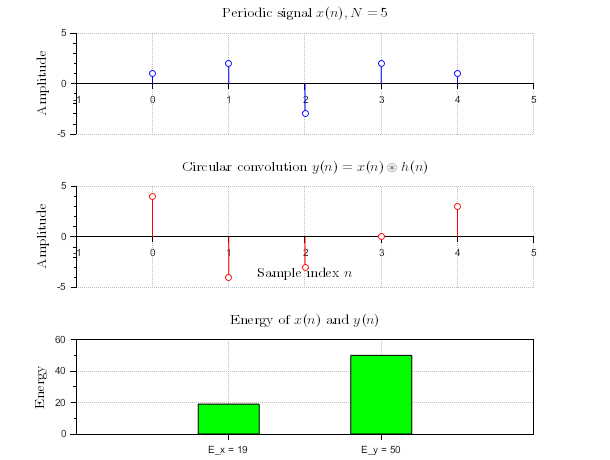
\includegraphics[width=0.85\linewidth]{ex4.7_0.png}
    \caption{Tín hiệu tuần hoàn $x(n)$, tích chập vòng $y(n)$ và năng lượng của hai tín hiệu}
    \label{fig:ex47}
\end{figure}

Cả hai phương pháp đều cho $y(n) = [4, -4, -3, 0, 3]$, khớp với bảng tính tay. Khác với Bài tập 6, ở đây $y(n)$ có cùng chiều dài $N = 5$ với $x(n)$, vì các mẫu lẽ ra nằm ngoài đoạn $[0, 4]$ của tích chập tuyến tính đã quay vòng và cộng chồng lên đầu chu kỳ (hiện tượng \emph{aliasing} trong miền thời gian). Do đó tích chập vòng chỉ trùng với tích chập tuyến tính khi $N \ge L_x + L_h - 1$; muốn dùng FFT để tính tích chập tuyến tính thì phải bù 0 cho cả hai tín hiệu đủ chiều dài này. Năng lượng $E_y = 50$, khác với $E_y$ của tích chập tuyến tính ở Bài tập 6 vì đáp ứng xung và cách cộng chồng đều khác.

\section{Bàn Luận}
Các kết quả tính tay biến đổi Z ở Bài 1--3 cho thấy rõ vai trò của ROC: tín hiệu hữu hạn hội tụ gần như trên toàn mặt phẳng, tín hiệu nhân quả có ROC nằm ngoài cực lớn nhất, còn tín hiệu hai phía có ROC là vành khuyên giữa các cực. Ở phần Scilab, cả hai phương pháp tích chập (gập--dịch và ma trận) đều cho kết quả trùng nhau và trùng với hàm \texttt{conv}. Qua Bài 7 em cũng hiểu vì sao tích chập vòng khác tích chập tuyến tính: các mẫu bị quay vòng và cộng chồng. Với dữ liệu thật, Scilab đọc và phân tích được phổ của tiếng mèo grừ, còn các phép cân bằng histogram, làm mờ và watermark trên ảnh đều cho kết quả đúng như mong đợi. Khó khăn em gặp là Scilab không đọc được file \texttt{.mp3} và ảnh khi chưa cài toolbox, nên em phải chuyển âm thanh sang \texttt{.wav} và tự viết hàm đọc ảnh PGM để script chạy được trên mọi máy.

\section{Tài Liệu Tham Khảo}
Đường link GitHub chứa mã nguồn thực hành source code SciLab: \url{https://github.com/qanetta/DigitalSignalProcessing-Lab.git}

\end{document}
